\documentclass[11pt]{article}
\usepackage[document]{ragged2e}
\usepackage[letterpaper, margin = 1in]{geometry}
\usepackage[utf8]{inputenc}
\usepackage{parskip}
\usepackage{circuitikz}
\usepackage{mathtools}
\usepackage{graphicx}
\usepackage{amsmath}
\usepackage{physics}
\usepackage{epstopdf}
\usepackage{indentfirst}
\usepackage{multicol}
\setlength{\columnsep}{1cm}
\usepackage{wrapfig}
\usepackage{subcaption}
\usepackage{siunitx}

\begin{document}
\centering
\textit{Summer Research 2019 Notes}\\
\textbf{Direct application of Bayesian inference on dynamic light scattering experiments to infer discretized particle size distribution}\\
Thy Doan Mai Le

\justifying
\section{Introduction}
Write about dynamic light scattering, why we're doing this, applications, what I'm trying to do specifically, previous works by other groups

\section{Testing Notes}
With an implementation of the $g^{(2)}$ function, a Gaussian distribution, a bidisperse distribution as well as a single point distribution of particle sizes were used to test the validity of the $g^{(2)}$ function's implementation. 
\subsection{Bidisperse Distribution}
The following self-generated particle size distribution with two peaks of different full-width-half-max (FWHM) values was used to test the validity of the $g^{(2)}$ function on a bimodal distribution. The reason for this test is to verify that the implementation written is able to work with a bimodal size distribution, since one of the advantages of the Direct Bayesian Method (DBM) is that it is able to work with almost any particle size distribution. 

\begin{figure}[h]
\centering
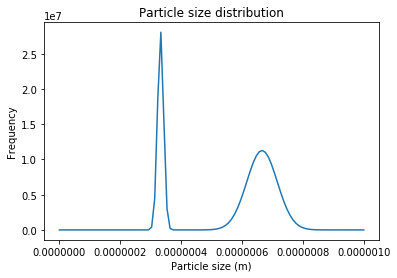
\includegraphics[width=0.5\linewidth]{bidisperse_psd.png}
\caption{The distribution of particle size (not normalized here) has a peak at $3.33\times10^{-7}$\si{meter} and another peak at $6.66\times10^{-7}$\si{meter}}
\label{fig:bidisperse_psd}
\end{figure}

From this distribution, the $g^{(2)}$ autocorrelation function of intensity v. time was found to be:

\begin{figure}[h]
\centering
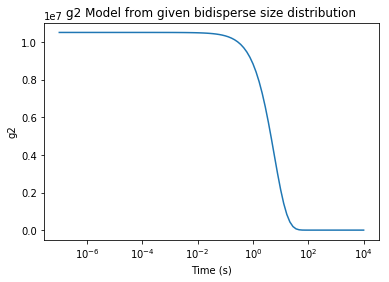
\includegraphics[width=0.5\linewidth]{g2.png}
\caption{The $g^{(2)}$ autocorrelation function extrapolated from the implementation.}
\label{fig:g2_model}
\end{figure}

In order to verify the validity of this autocorrelation function, I used SciPy's optimization for curve fits to extrapolate, from this autocorrelation function, the single exponential decay and the method of cummulants models. The goal of this method of testing is to verify that both of the single exponential decay and cummulants models fail upon the emergence of a bimodal particle size distribution. In order to detect this anticipated failure, the residuals between the $g^{(2)}$ model and each of the tested models (single exponential/cummulants) are plotted. Failure of each of the tested models is present when overshooting and/or undershooting are present in the residuals plot. 

When tested against the single exponential decay model, the residuals plot is as follows:

\begin{figure}[h!]
\centering
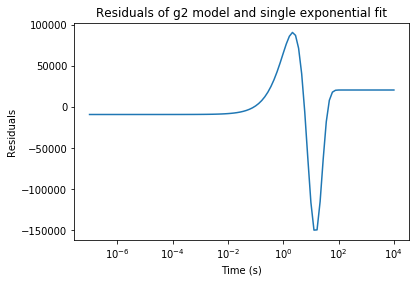
\includegraphics[width=0.5\linewidth]{expo_residuals.png}
\caption{The undershooting and overshooting are both apparent around the region of exponential decay, implying that the exponential fit is unable to capture certain aspects of the autocorrelation. This is congruent with the given data. Since single exponentials are only able to capture information of systems with 1 single particle size, a bimodal distribution of particle size should render the single exponential model inept.}
\label{fig:expo_residuals}
\end{figure}

When tested against the cummulants model, the residuals plot is as follows:

\begin{figure}[h!]
\centering
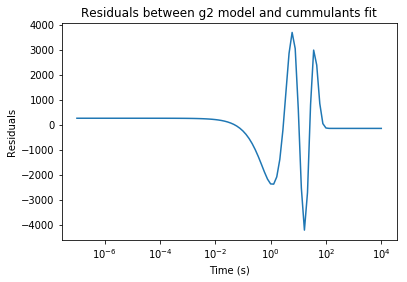
\includegraphics[width=0.5\linewidth]{cummulants_fit_residuals.png}
\caption{The residuals between the autocorrelation and the cummulants fit model showed dramatic breakdown around the exponential decay region, signifying that the cummulants fit was not able to truly capture the $g^{(2)}$ information.}
\label{fig:cummulants_residuals}
\end{figure}

In conclusion, the residuals plots have shown that both the single exponential and the cummulants model were unable to fully capture the information displayed in the $g^{(2)}$ autocorrelation and therefore should not be used in analyzing dynamic light scattering information of samples with know multimodal particle size distributions. 

\subsection{Single Gaussian distribution}
Write about tests of the g(2) model using a single Gaussian distribution of particle sizes. In this test, the expected results are that the method of cumulants and the single exponential model both fail to completely capture the physics, shown by a residual plot that exhibits overshooting and undershooting of results.

\section{Derivation of Bayesian distributions}
\subsection{Prior Distribution}
According to Buoalem, Jabloun, Ravier, Naiim and Jalocha, the prior distribution of this non-parametrized method is as follows:

\begin{equation}\label{eq:prior}
p(\mathbf{f}) \propto exp\left( \mathbf{f}^{T} \mathbf{L_2}^{T}\mathbf{L_2}\mathbf{f} \right), \textrm{if } \mathbf{g} \geq 0
\end{equation}

\subsection{Likelihood Distribution}
The likelihood distribution is modeled according to the $g^{(2)}$ function as 

\begin{equation} \label{eq:likelihood}
p(\mathbf{\tilde{g}^{(2)}} | \mathbf{f}, \sigma^{2}_r ) = \frac{1}{{(2\pi)}^{\frac{M_r}{2}} \sigma^{M_r}}exp\left( -\frac{\chi_r(\mathbf{f})}{2\sigma^2_r}\right)
\end{equation}
if $\mathbf{f} \geq 0$.

The $\chi$-squared $\chi_r(\mathbf{f})$ is defined as 

\begin{equation}
\chi_r(\mathbf{f}) = \sum_{j=1}^{M_r} {\left( \tilde{g}_{\theta_r}^{(2)} (\tau_j) - g_{\theta_r}^{(2)} (\tau_j) \right)}^2
\end{equation}

\subsection{Posterior Distribution}
With the prior and likelihood distributions described in Eq.~\ref{eq:prior} and Eq.~\ref{eq:likelihood}, the posterior distribution for the particle size distribution with the noise variance given the measured autocorrelation data ($g^{(2)}$) is: 

\begin{equation}\label{eq:posterior}
p(\mathbf{f}, \sigma_1^2,\ldots, \sigma_r^2|\mathbf{\tilde{g}^{(2)}}) \propto exp \left( -\mathbf{f}^T\mathbf{L_2}^T\mathbf{L_2} \right) \prod_{r=1}^{R} \left[ \frac{1}{\sigma_r^{M_r+2}} exp \left( -\frac{\chi_r(\mathbf{f})}{2\sigma_r^2} \right) \right]
\end{equation}

Using the classical Jeffrey prior density for the noise variance in $\mathbf{\tilde{g}^{(2)}}$,
\begin{equation}\label{eq:noisevariance}
p(\sigma_r^2) \propto \frac{1}{\sigma_r^2}
\end{equation}
the posterior distribution can be integrated over the noise variance with the following integral:

\begin{equation} \label{eq:originalIntegral}
\int_{0}^{\infty} \frac{1}{\sigma_r^{M_r + 2}} exp \left( -\frac{\chi_r(\mathbf{f})}{2\sigma_r^2} \right)d\sigma_r
\end{equation}
 
 In order to integrate this integral, let $\sigma_r = \frac{1}{t}$ and thus $d\sigma_r = -\frac{1}{t^2}dt$. From this, we can rewrite expressions from the integrand in Eq.~\ref{eq:originalIntegral} as follows.
  \begin{equation}
 \begin{split}
 \frac{1}{\sigma_R^{M_r + 2} } & = t^{M_r + 2} \\
 \frac{\chi_r(\mathbf{f})}{2\sigma_r^2} & = \frac{\chi_r(\mathbf{f})}{2} t^2
 \end{split}
 \end{equation}
 Thus the integral from Eq.~\ref{eq:originalIntegral} becomes:
 \begin{equation} \label{eq:substitution1}
 \begin{split}
&  \int_{\infty}^{0} t^{M_r + 2} \left( -\frac{1}{t^2} \right)exp \left( -\frac{\chi_r(\mathbf{f})}{2} t^2 \right) dt \\
& =  \int_{0}^{\infty} t^{M_r}exp\left( -\frac{\chi_r(\mathbf{f})}{2} t^2 \right) dt
 \end{split}
 \end{equation}
 The limits switched from (0, $\infty$) in Eq.~\ref{eq:originalIntegral} to ($\infty$, 0) in Eq.~\ref{eq:substitution1} because of the substitution $\sigma_r = \frac{1}{t}$. The reciprocal relationship of the substitution switched the limits of the integration. In order to make the integral easier to integrate, the minus sign on the second line of Eq.~\ref{eq:substitution1} is exchanged for the re-switching of the integration limits from ($\infty$, 0) back to (0, $\infty$). 
 
 In order to actually integrate Eq.~\ref{eq:substitution1}, a second substitution has to be made. Let $\tau = t\sqrt{\chi_r}$ and d$\tau = \sqrt{\tau}$dt. From this, we can rewrite the expressions in the integrand of Eq.~\ref{eq:substitution1} as follows. 
 \begin{equation}
 \begin{split}
 \chi_r(\mathbf{f}) t^2 & = \tau^2 \\
 t^{M_r} & = {\left( \frac{\tau}{\sqrt{\chi_r}} \right)}^M_r \\
 & = \tau^{M_r}\chi_r^{-\frac{M_r}{2}} 
 \end{split}
 \end{equation}
 
 From the above substitutions, the integral becomes:
\begin{equation}
\begin{split}
 & \int_{0}^{\infty}\chi_r^{-\frac{1}{2}} \tau^{M_r} \chi_r^{-\frac{M_r}{2}} exp\left( -\frac{\tau^2}{2} \right) d\tau \\
& = \int_{0}^{\infty} \chi_r^{-\frac{1}{2}(M_r + 1)} \tau^{M_r} exp\left( -\frac{\tau^2}{2} \right) d\tau
\end{split}
\end{equation}

Since the $\chi_r$ term does not have $\tau$ dependence, we can pull that out of the integrand, giving us the following integral at the end:
\begin{equation}
\chi_r^{-\frac{1}{2}(M_r + 1) }\int_{0}^{\infty}\tau^{M_r}exp\left( -\frac{\tau^2}{2} \right) d\tau
\end{equation}

Recall that the $\chi_r$ expression was previously 
\begin{equation}
\chi_r(\mathbf{f}) = \sum_{j=1}^{M_r} {\left( \tilde{g}^{(2)}_{\theta_r} (\tau_j) - g^{(2)}_{\theta_r}(\tau_j) \right)}^2
\end{equation}
where $\tilde{g}^{(2)}$ is modeled to be:
\begin{equation}
\begin{split}
 \tilde{g}^{(2)}_{\theta_r} (\tau_j) & = 1 + \beta_r {\left( k_{\theta_r}\sum_{i=1}^{N}f(D_i) C_{I,\theta_r}(D_i) exp\left( -\frac{\Gamma_{0,\theta_r}}{D} \tau_j \right) \Delta D_i \right)}^2 \\
\text{where } \Gamma_{0,\theta_r} & = \frac{16\pi n^2 \sin^2(\theta/2)k_B T}{2\lambda_0^2\eta}
 \end{split}
\end{equation}

with 

\begin{equation}
\begin{split}
& \text{n } : \text{refractive index}\\
& \theta\text{ : angle at which scattered light was measured}\\
& k_B\text{ : Boltzmann constant} \\
& T\text{ : temperature in Kelvin} \\
& \lambda_0\text{ : incident wavelength value in vacuum}\\
& \eta\text{ : viscosity} \\
& D_i\text{ : diameter of particle size}\\
& \beta_r\text{ : instrumental factor}\\
& k_{\theta_r}\text{ : normalization constant that can be found via k = }\frac{1}{\int_{0}^{\infty} f(D)C_{I,\theta}(D) dD}\\
&\tau_j\text{ : delay times} \\
&f(D)\text{ : the particle size distribution function}
\end{split}
\end{equation}

The posterior distribution is now defined to be:
\begin{equation}
p(\mathbf{f}|\tilde{\mathbf{g}}^{(2)}) \propto exp\left( -\mathbf{f}^T\mathbf{L_2}^T \mathbf{L_2}\mathbf{f}\right) \prod_{r=1}^{R} {\left[\chi_r(\mathbf{f})\right]}^{-\frac{M_r}{2}}
\end{equation}

Since $\chi_r(\mathbf{f}) = \sum {\left( \tilde{g}^{(2)}_{\theta_r} (\tau_j) - g^{(2)}_{\theta_r}(\tau_j) \right)}^2$, the posterior distribution is essentially:
\begin{equation}
p(\mathbf{f}|\tilde{\mathbf{g}}^{(2)}) \propto exp\left( -\mathbf{f}^T\mathbf{L_2}^T \mathbf{L_2}\mathbf{f}\right) \prod_{r=1}^{R} {\left( \sum{(\tilde{g}^{(2)}_{\theta_r} (\tau_j) - g^{(2)}_{\theta_r}(\tau_j) )}^2 \right)}^{-\frac{M_r}{2}}
\end{equation}

When the log of the posterior is taken, the above equation becomes:
\begin{equation}
\ln(p) = -\mathbf{f}^T\mathbf{L_2}^T \mathbf{L_2}\mathbf{f} + \left(-\frac{M_r}{2} \right) \ln \left(\sum {\left( \tilde{g}^{(2)}_{\theta_r} (\tau_j) - g^{(2)}_{\theta_r} (\tau_j) \right)}^2 \right)
\end{equation}

%%%%%%%%%%%%%%%%%%%%%%%%%%%%%%%%%%%%%%%%%%%%%%%%%%%%%%%%
% Actual Testing 
% with 2015_07_22_Eonly0005 asc data
%%%%%%%%%%%%%%%%%%%%%%%%%%%%%%%%%%%%%%%%%%%%%%%%%%%%%%%%

\section{Testing Round 1 - 06/24/2019}
The current code on github was used to infer the discretized particle size distribution of the data gathered in a data file which was collected by Professor Jerome Fung. 

The emcee algorithm requires that starting positions be given for the walkers such that the walkers would be closest to the most probable values that are about to be inferred. In previous methods, such as Bayesian inference with the method of cumulants, the most probably values can be estimated using least square fitting. Therefore, in this testing round, the same procedure for finding the most probable values for the walkers' starting positions is used. The starting position is first extracted from the raw data using least square fitting to find the most likely particle radius size. Then, since we already know that this particular data came from a sample that has unimodal size distribution, a Gaussian distribution is generated with a mean being the most likely particle radius size. The distribution is also normalized prior to Bayesian inference. 

The most probable particle radius size was found to be 2.2439$\times10^{-9}$\si{meter}. From this most probably size, a Gaussian particle size distribution was generated to be Fig.~\ref{fig:f}

\begin{figure}[h!]
\centering
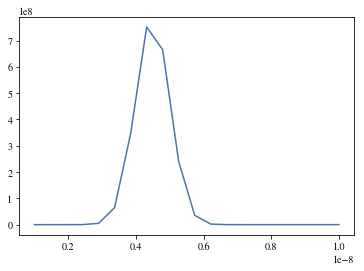
\includegraphics[width=0.5\linewidth]{theory_f(D)_06242019.png}
\caption{The theoretical particle size distribution that was generated from the least-square fitting of the raw data has a mean of 4.4878$\times10^{-9}$\si{meter} and a standard deviation of 5$\times10^{-10}$\si{meter}.}
\label{fig:f}
\end{figure}

With this particle size distribution as the starting position, the actual particle distribution was inferred using the Bayesian method to be as described in Fig.~\ref{fig:actual_distribution1}.

\begin{figure}[h!]
\centering
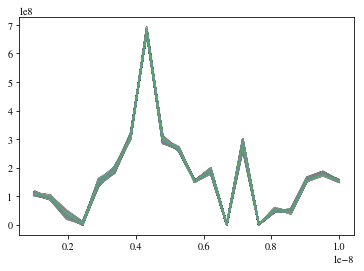
\includegraphics[width=0.5\linewidth]{f(D)_06242019.png}
\caption{The inferred particle size distribution that was generated using Bayesian inference on the raw data file aforementioned, using the generated particle size distribution in Fig.~\ref{fig:f} as starting positions.}
\label{fig:actual_distribution1}
\end{figure}

\end{document}